\subsection{Parameter Identification}
Fig. \ref{fig:length_pressure} displays the relationship between the pressure $p$ and the natural length $l_n$ of the PAMs. As assumed, there is a tendency for $l_n$ to decrease linearly with $p$ within the range of the tested pressure. The dashed lines in Fig. \ref{fig:length_pressure} represent the fitted lines using the least squares method, expressed by Eq. (\ref{eq:L_n}).
Fig. \ref{fig:pam_b_static1} shows the result of the static loading experiment for PAM-B. The red and blue points represent the data during expansion and contraction respectively, and the green dashed lines represent the solutions $d$ to Eq. (\ref{eq:model}), which is given by substituting the acquired parameters $a_i$ and the measured $f$ and $p$.
Generally, PAMs exhibit hysteresis due to friction, so the data differ between expansion and contraction processes. We only present the static loading experimental result for PAM-B because of the space constraint, but similar results were obtained for the other PAMs.

\begin{figure}[t]
    \hfill
    \begin{minipage}{\columnwidth}
        \centering
        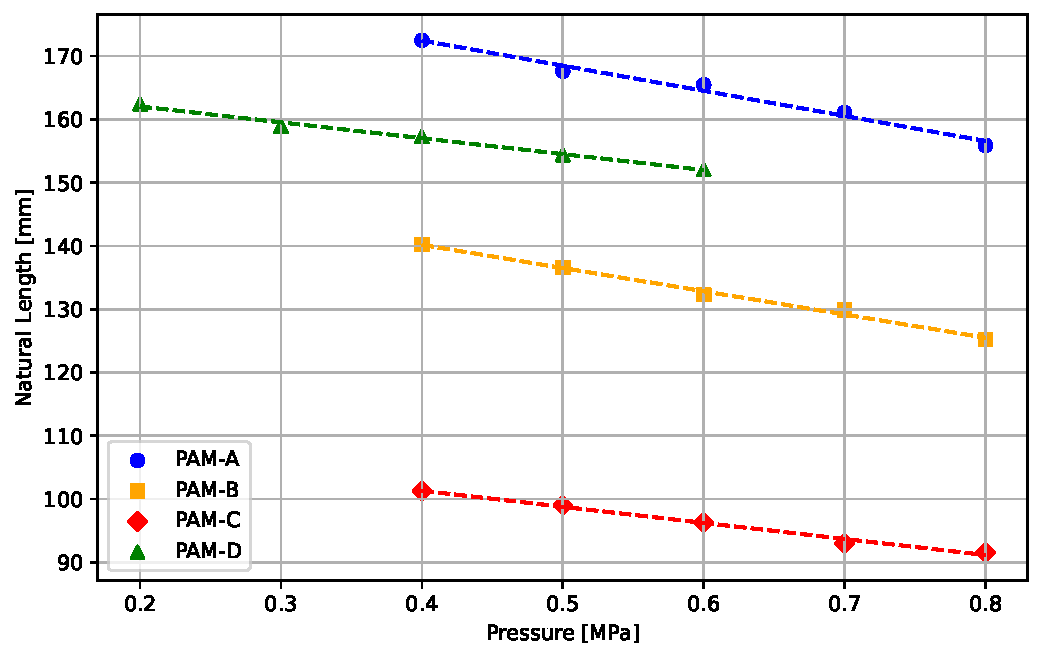
\includegraphics[width=\columnwidth]{fig/length_pressure.pdf} 
        \caption{Relationship between Pressure and Natural Length}
        \label{fig:length_pressure}
        \vspace{1em} 
        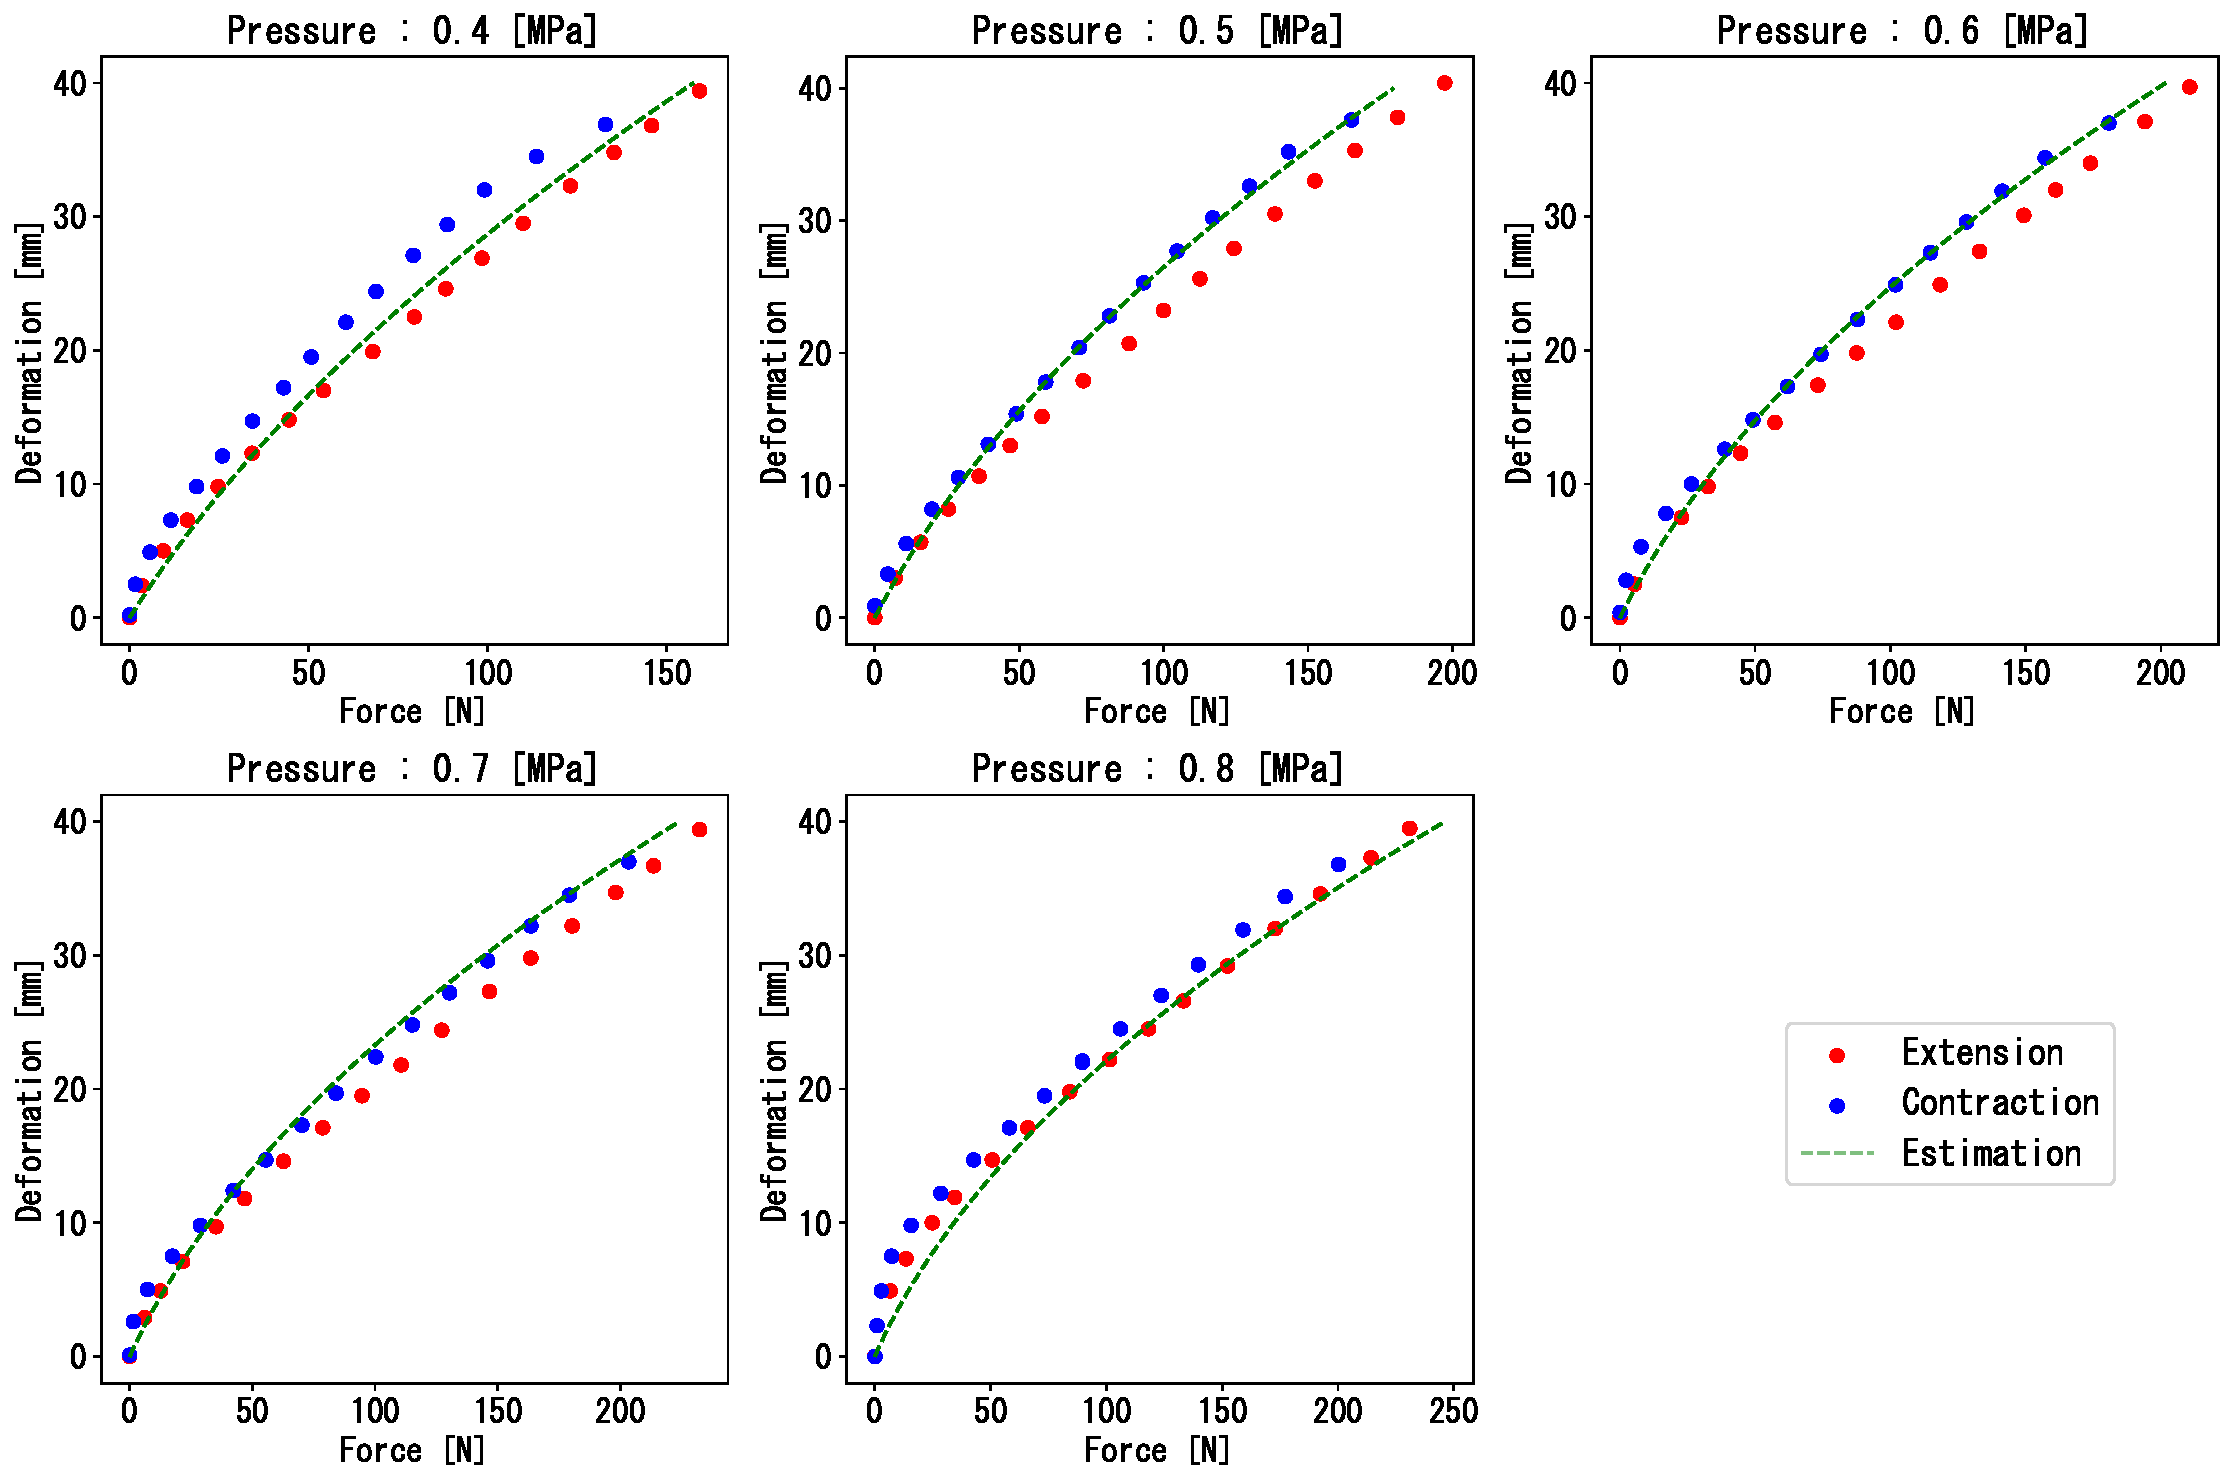
\includegraphics[width=\columnwidth]{fig/20231124_5_4s_2d_ieeesensors1.pdf}
        \caption{Relationship between Force and Deformation at Each Pressure (PAM-B)}
        \label{fig:pam_b_static1}
    \end{minipage}
    \hspace{0.05\textwidth} 
\end{figure}




% \begin{textblock*}{\columnwidth}(11cm,3cm) 
% \begin{figure}
%     \centering
%     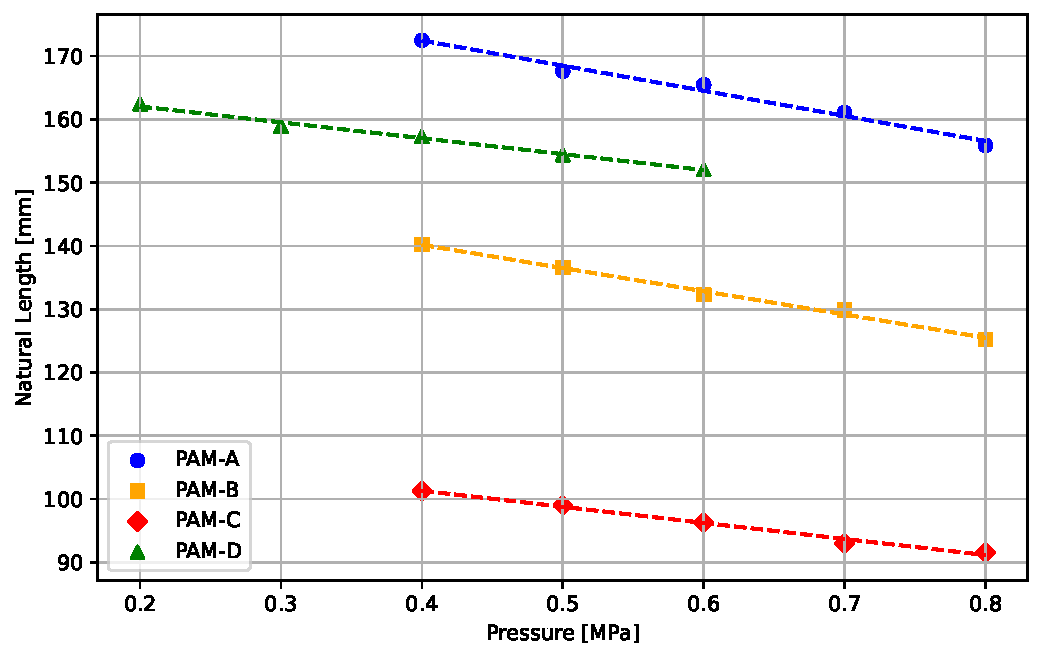
\includegraphics[width=\columnwidth]{fig/length_pressure.pdf}
%     \caption{Relationship between Pressure and Natural Length}
%     \label{fig:length_pressure}
% \end{figure}
% \end{textblock*}


% \begin{textblock*}{\columnwidth}(11cm,12cm) 
% \begin{figure}
%    \centering
%    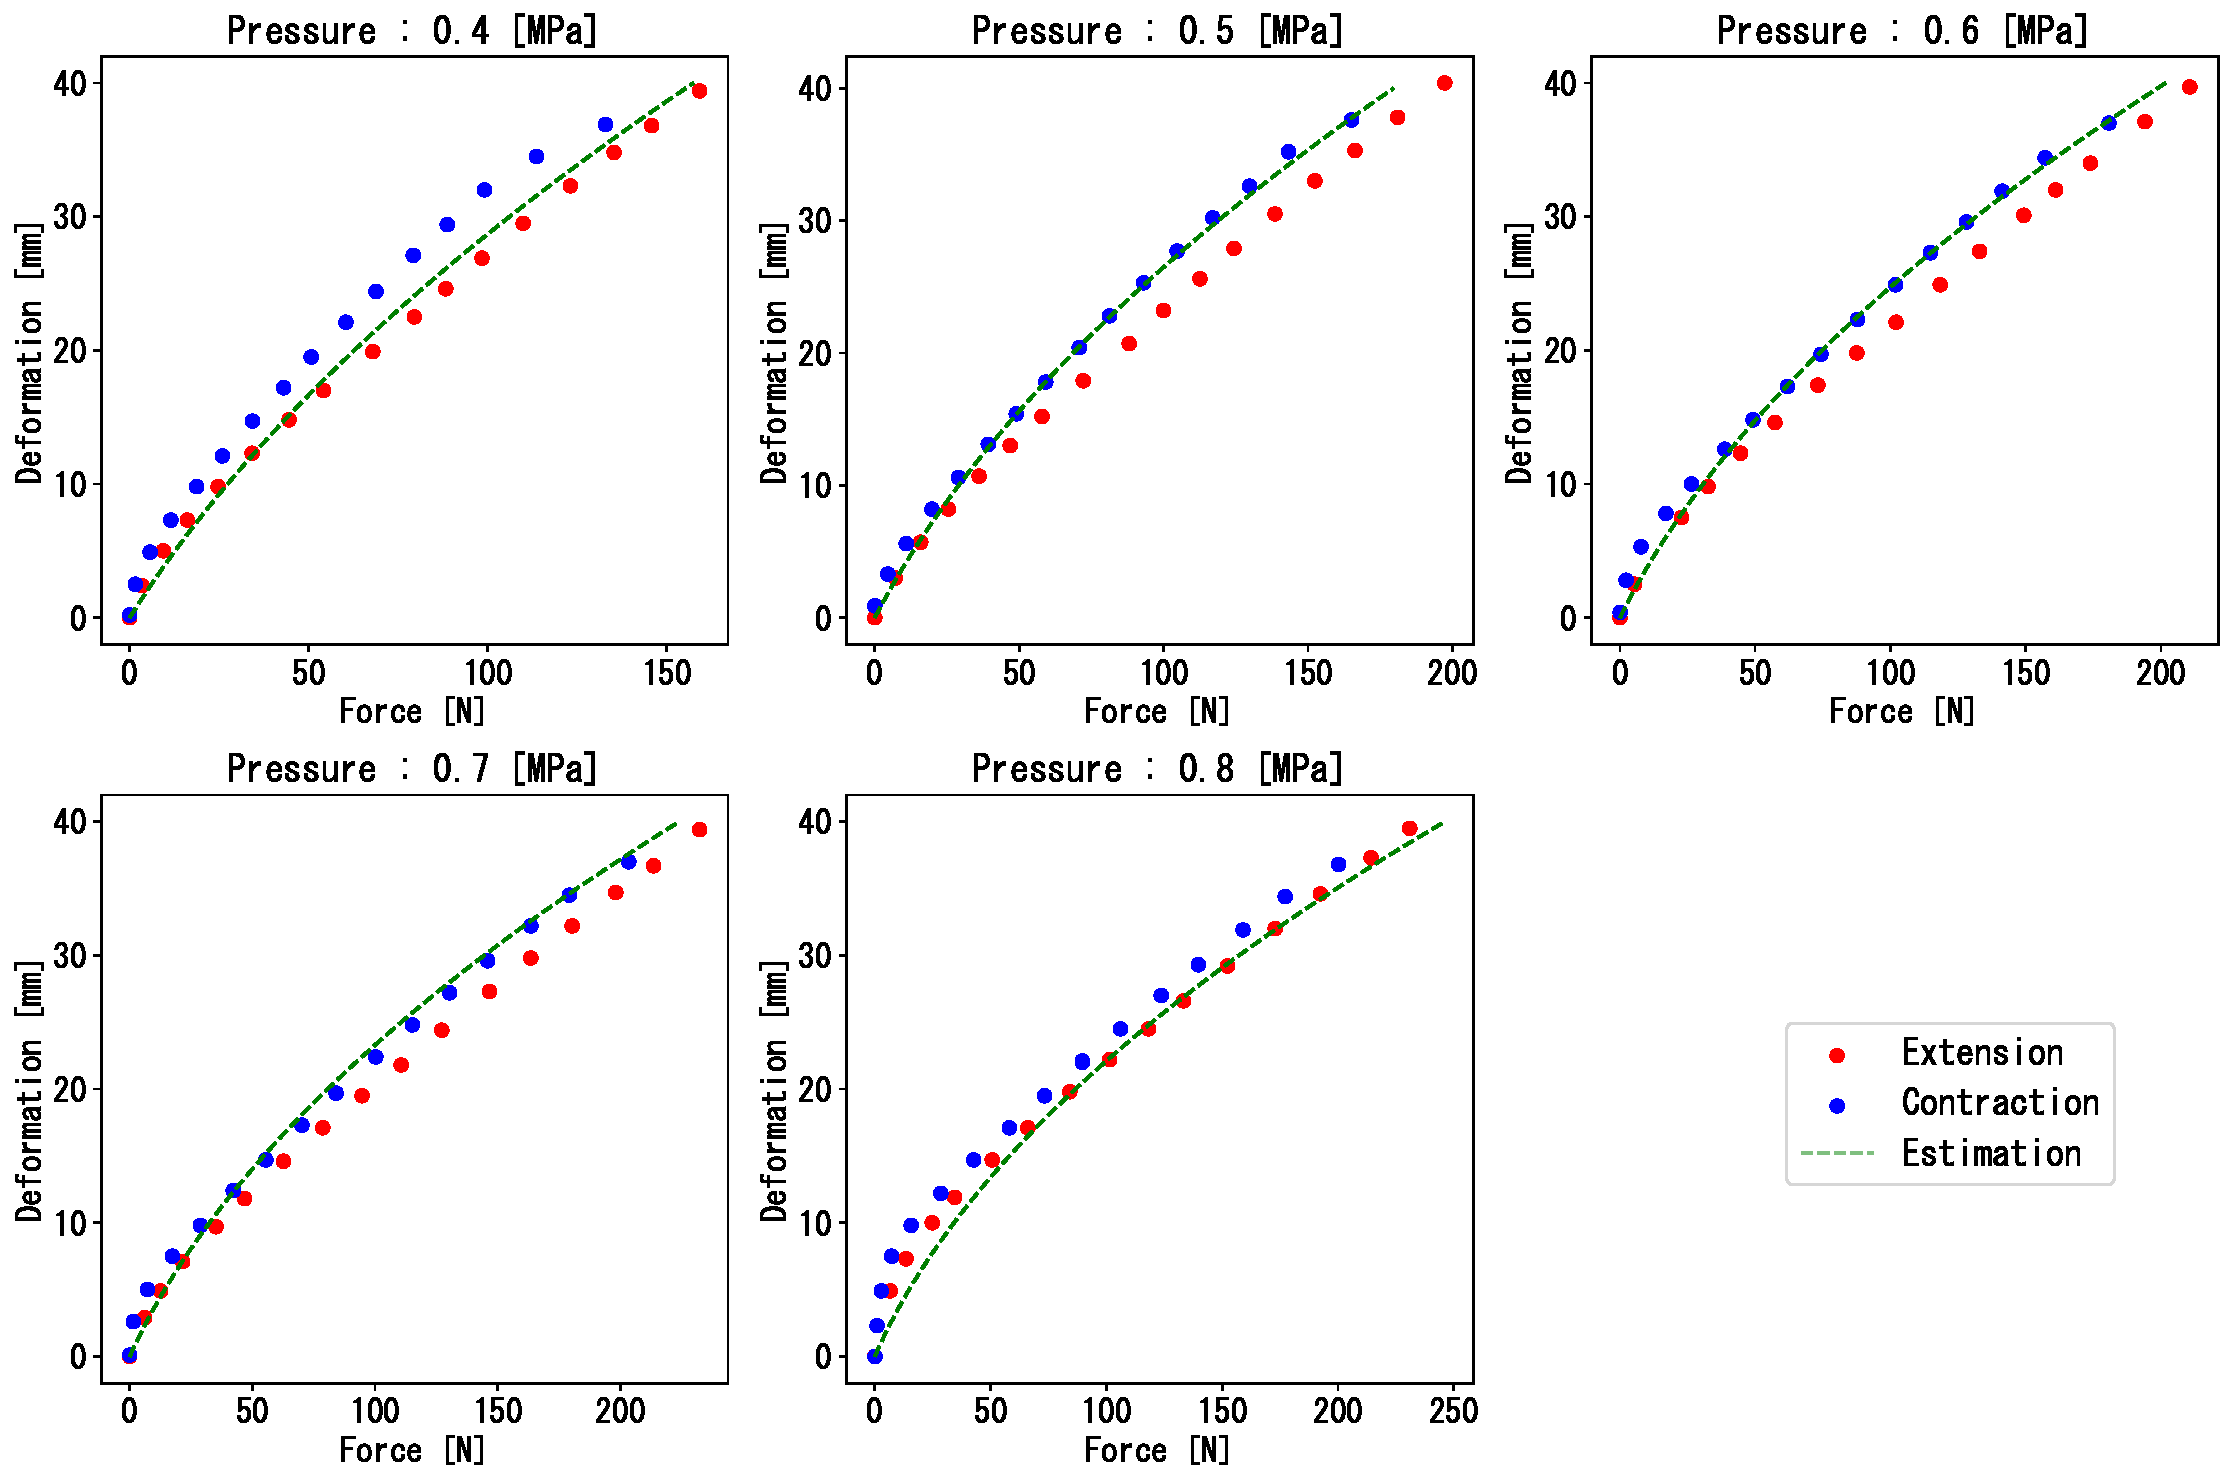
\includegraphics[width=\columnwidth]{fig/20231124_5_4s_2d_ieeesensors1.pdf}
%    \caption{Relationship between Force and Deformation at Each Pressure (PAM-B)}
%    \label{fig:pam_b_static1}
% \end{figure}
% \end{textblock*}

% % 画像にかからないようにテキスト位置を調整
% \vspace{40cm} % 必要に応じて調整してください

% \begin{figure}[H]
%     \centering
%     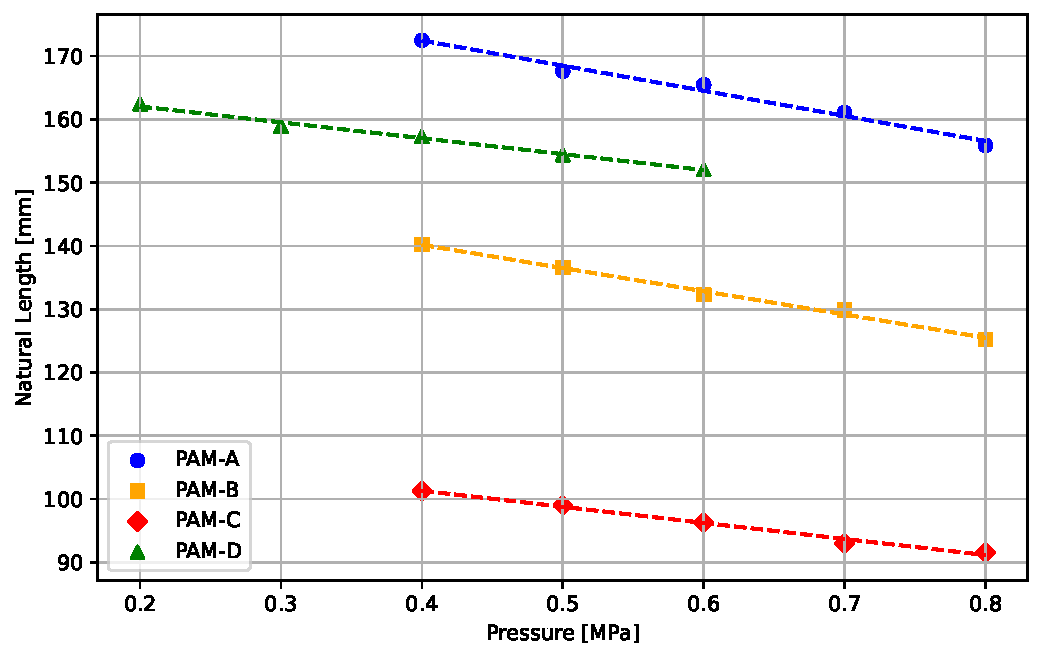
\includegraphics[width=\columnwidth]{fig/length_pressure.pdf}
%     \caption{Relationship between Pressure and Natural Length}
%     \label{fig:length_pressure}
% \end{figure}

% \begin{figure}[H]
%    \centering
%    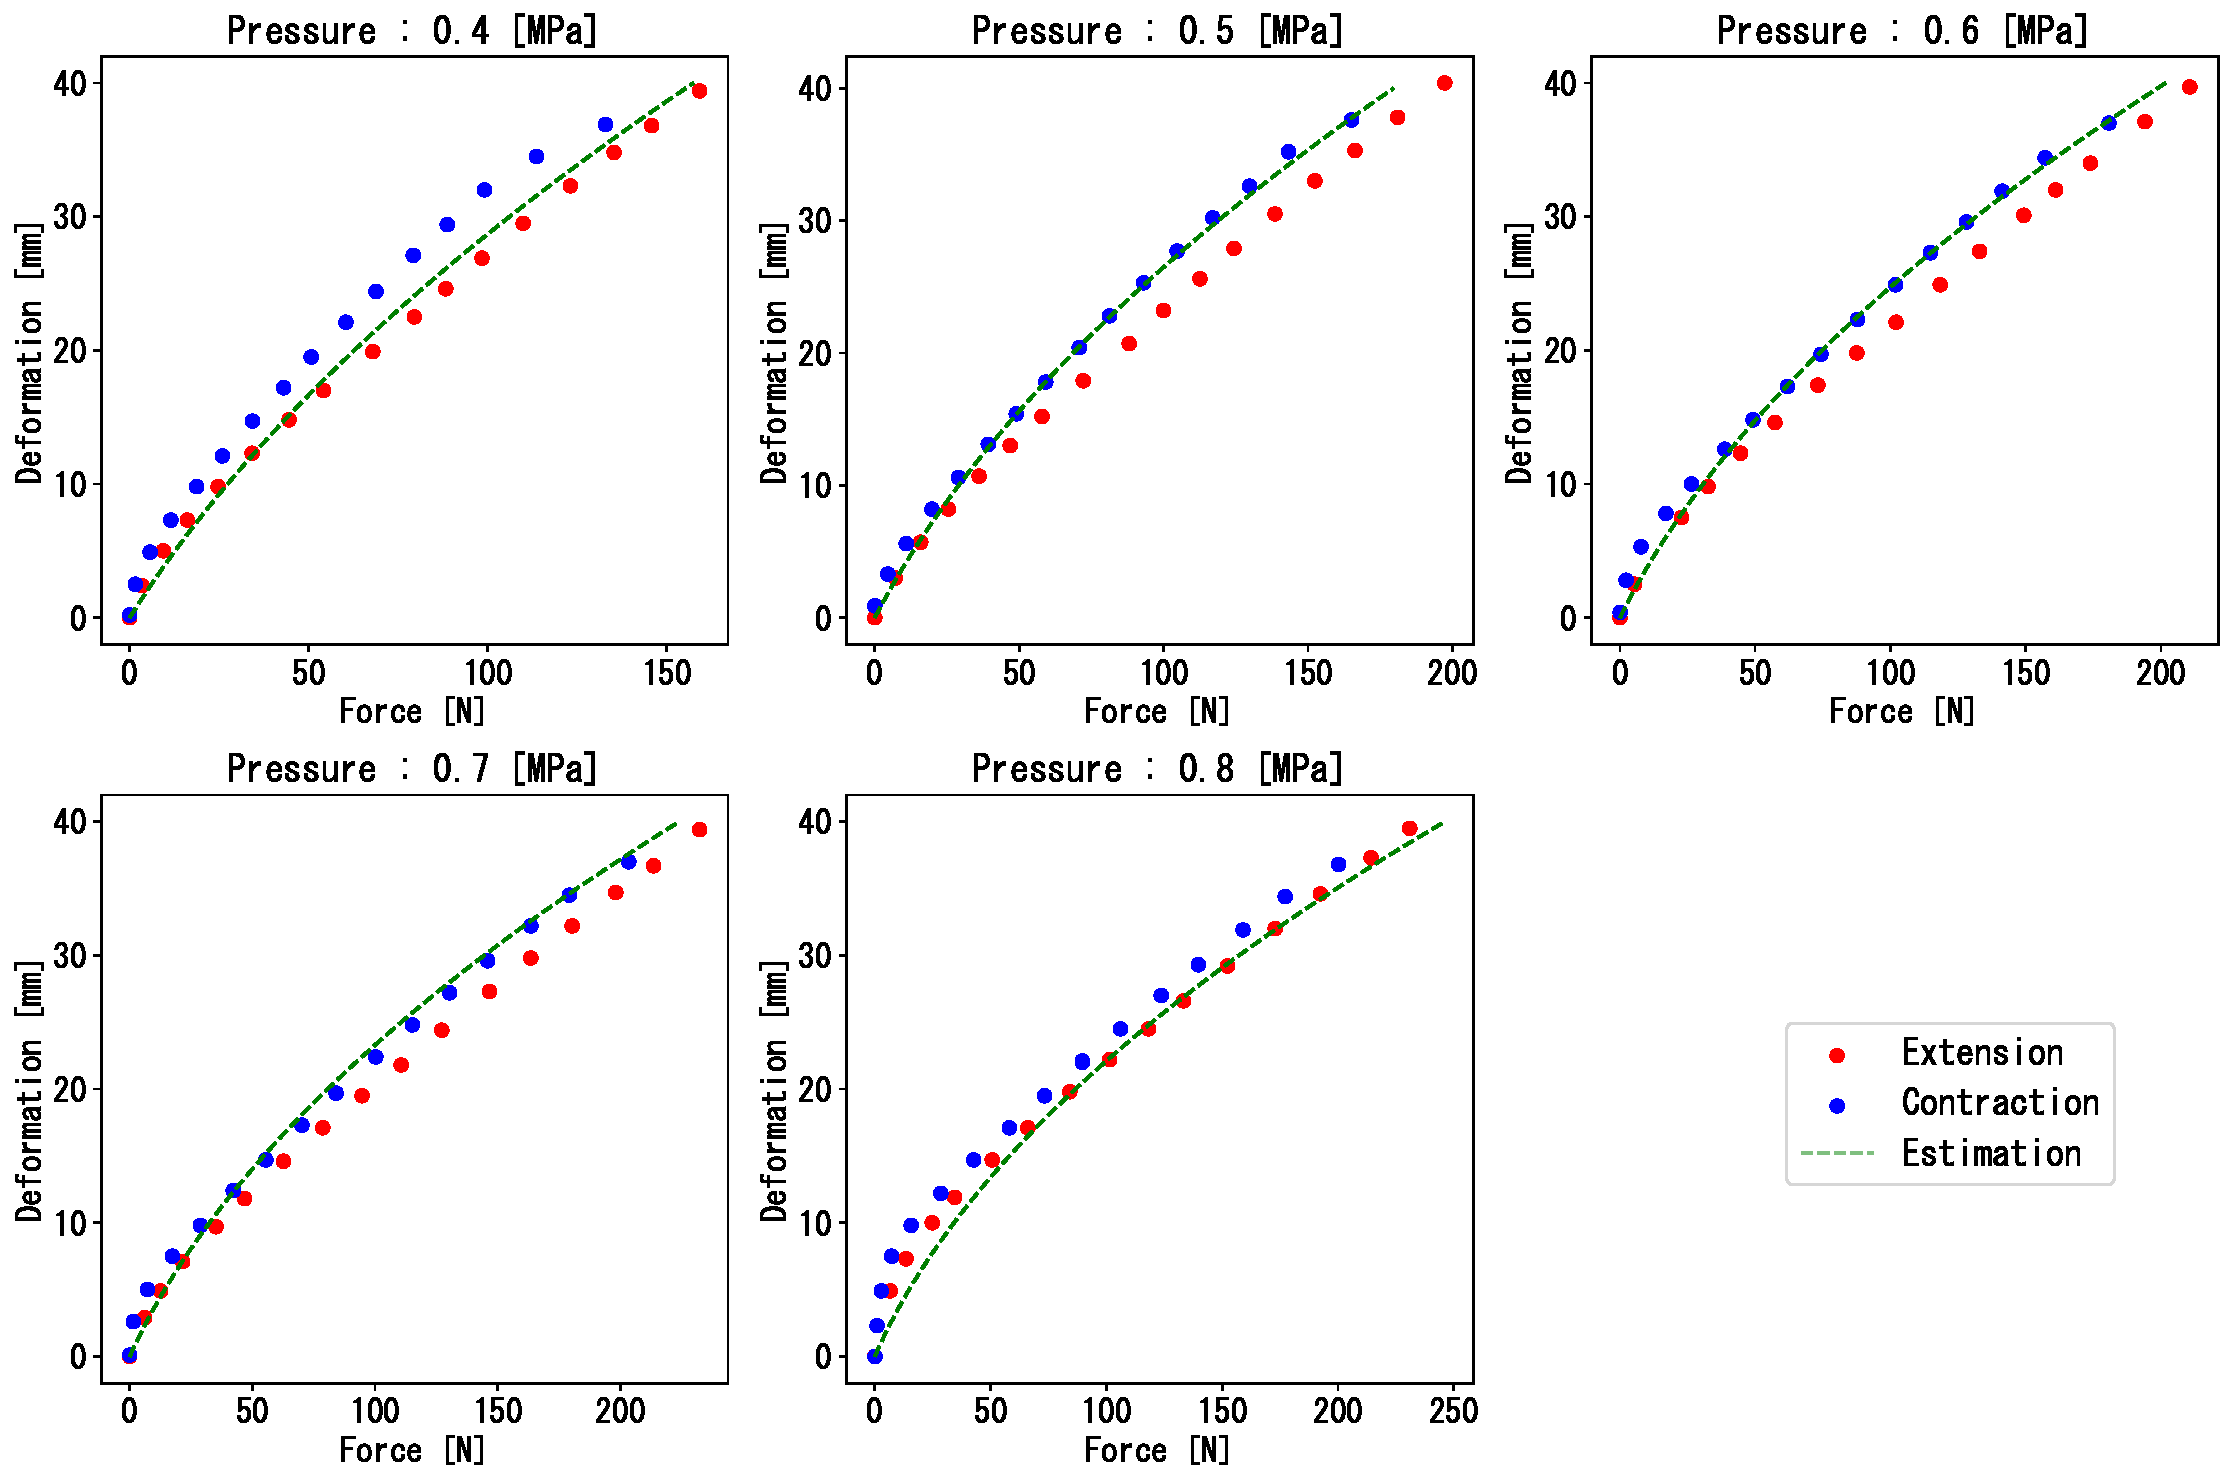
\includegraphics[width=\columnwidth]{fig/20231124_5_4s_2d_ieeesensors1.pdf}
%    \caption{Relationship between Force and Deformation at Each Pressure (PAM-B)}
%    \label{fig:pam_b_static1}
% \end{figure}


\begin{figure*}[h]
   \begin{center}
       \begin{minipage}[t]{\columnwidth} 
           \centering
           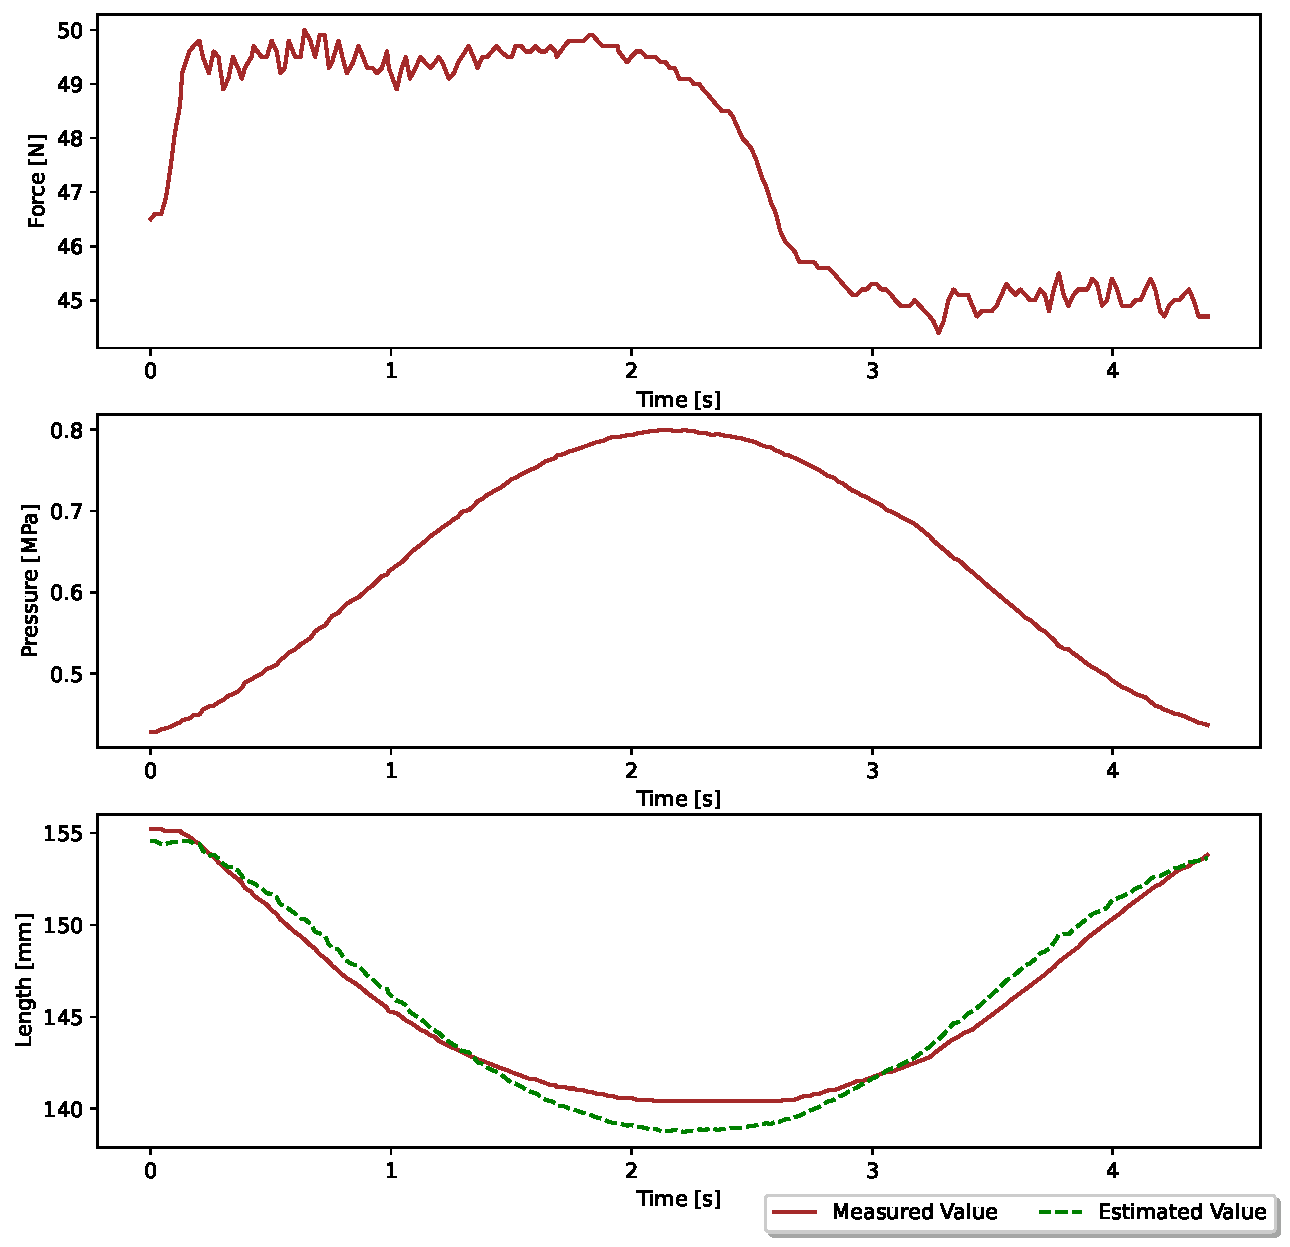
\includegraphics[keepaspectratio, width=\columnwidth]{fig/20231207_1_4s_by_5_2d_ieeesensors1.pdf}
           \caption{Dynamic Length Estimation (PAM-B, Rubber)}
           \label{fig:pam_b_dynamic}
       \end{minipage}
       \hfill
       \begin{minipage}[t]{\columnwidth} 
           \centering
           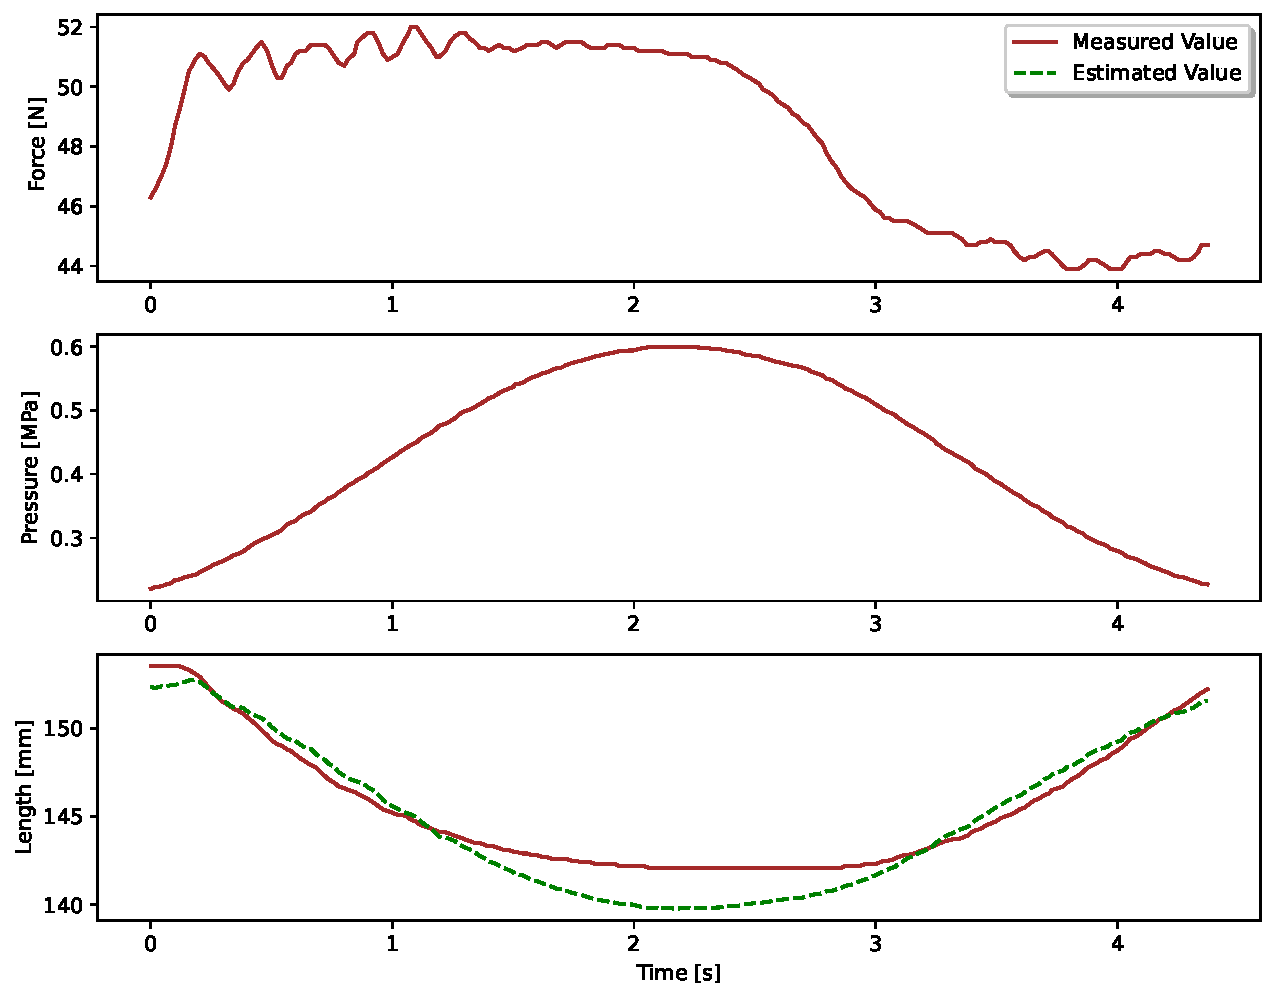
\includegraphics[keepaspectratio, width=\columnwidth]{fig/20231220_2_s_by_2_2d_ieeesensors1.pdf}
           \caption{Dynamic Length Estimation (PAM-D, Silicon)}
           \label{fig:pam_d_dynamic}
       \end{minipage}
   \end{center}
\end{figure*}

\vspace{1cm}

% \begin{figure}[H]
%    \centering
%    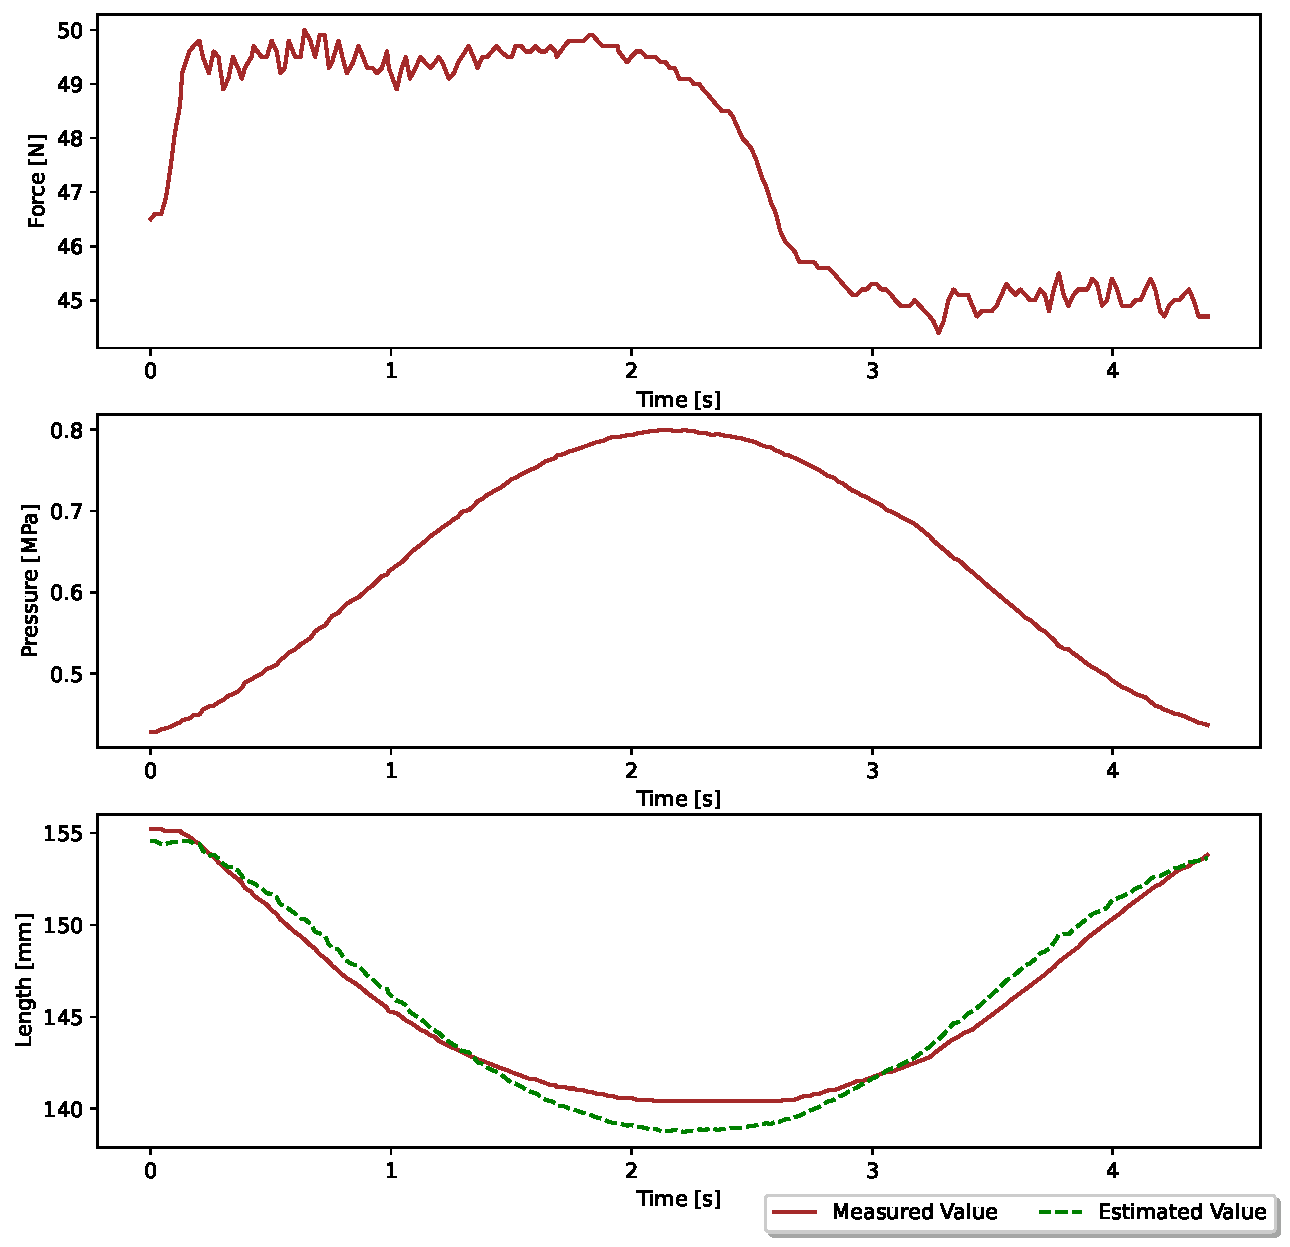
\includegraphics[width=\columnwidth]{fig/20231207_1_4s_by_5_2d_ieeesensors1.pdf}
%    \caption{Dynamic length estimation (PAM-B, Rubber)}
%    \label{fig:pam_b_dynamic}
% \end{figure}
\subsection{Error Evaluation} 
Fig. \ref{fig:pam_b_dynamic} and Fig. \ref{fig:pam_d_dynamic} show the dynamic length estimation result for PAM-B and PAM-D, respectively.
With the proposed method, with respect to the measurements by the linear encoder, the length estimation was achieved with maximum errors of $1.72\%$ for PAM-A, $1.19\%$ for PAM-B, $1.18\%$ for PAM-B, and  $1.65\%$ for PAM-D respectively , and with root mean squared errors of $0.861\%$ for PAM-A, $0.653\%$ for PAM-B, $0.683\%$ for PAM-C, and $0.846\%$ for PAM-D respectively.

\subsection{Reaching Task}
Table. \ref{tab:PAM_reflex} shows the parameters for the length estimation of the agonist and antagonist muscles. The considerable difference in the voltage-force slope $q$ between the two PAMs is attributable to the varying sensitivities of the handmade strain gauges.

Fig.\ref{fig:reaching_error} displays the length estimation errors of the model and the fiber sensor in reaching task. Since the fiber sensor could only measure the rate of length change and not the absolute length, the estimated absolute length by the fiber sensor was calibrated to the measurement value from the linear encoder at the start of the reaching task. Therefore, it cannot be said that Fig.\ref{fig:reaching_error} is exactly comparing the estimates from the model and from the fiber sensor, but it serves as a reference for examining the accuracy of the model against the conventional sensor. The reaching task was performed five times for both the agonist and antagonist muscles. For the agonist muscle, with respect to the linear encoder measurement, the model showed a maximum error of $5.86\%$ and a root mean squared error of $3.17\%$, while the fiber sensor showed a maximum error of $2.53\%$ and a root mean squared error of $1.02\%$. For the antagonist muscle, the model showed a maximum error of $5.86\%$ and a root mean squared error of $5.02\%$, while the fiber sensor showed a maximum error of $2.53\%$ and a root mean squared error of $1.78\%$. 

\begin{table}[H]
    \centering
    \caption{Parameters for Length Estimation} 
    \resizebox{\columnwidth}{!}{%
    \begin{tabular}{c|ccccccc}
        \hline
        PAM & $m$ & $h$ & $a_3$ & $a_2$ & $a_1$ & $a_0$ & $q$ \\
        \hline \hline
        Agonist & -60.1 & 170.1 & -0.201 & 7.00 & 0.256 & 0.911 & $2.25 \times 10^{-3}$\\
        Antagonist & -70.3 & 178.5 & 0.871 & 1.24 & -0.129 & 22.4 & $4.33 \times 10^{-3}$ \\
        \hline
    \end{tabular}
    } 
    \label{tab:PAM_reflex}
\end{table}


\subsection{Stretch Reflex}
Table \ref{tab:reflex_para} shows the velocity threshold $V_{thr}$ and the feedback gain $k$, and they were determined experimentally by assessing the magnitude of the impact. 

\begin{table}[h]
    \centering
    \caption{Parameters for Stretch Reflex} 
    \begin{tabular}{c|cc}
        \hline
        PAM &$V_{thr} [\si{mm/s}]$&$ k [\si{GPa\cdot s}]$\\
        \hline \hline
        Model & 70 & 1/800\\
        Fiber Sensor & 25 & 1/300\\
        \hline
    \end{tabular}
\label{tab:reflex_para}
\end{table}

Fig. \ref{fig:reflex_all} illustrates the dynamic behavior of the reflex by the model. The starting angle of the arm was -36 deg due to the basket's weight of 83.1 g. When the falling mass made an impact, the angle dropped dramatically, creating sudden soar in the voltage signal from the strain gauge and thus in the estimated velocity. It went beyond the threshold and triggered the stretch reflex, leading to increasing pressure in the agonist muscle and decreasing in antagonist. The arm was then lifted back to the initial position, and after some oscillation, it settled down to a certain angle, holding the mass left in the basket.

Fig.\ref{fig:reflex_angle} displays the average and range of angles in 20 trials of the reflexes by the model and by the fiber sensor.

それぞれの反射に対して、閾値やゲインを実験的に決めているので、純粋にアームの角度の振る舞いを比較することはできないが、ファイバーセンサによる反射をモデルにより再現できていると言える。高橋らは、伸張反射のみならず、

% \begin{figure}[H]
%    \centering
%    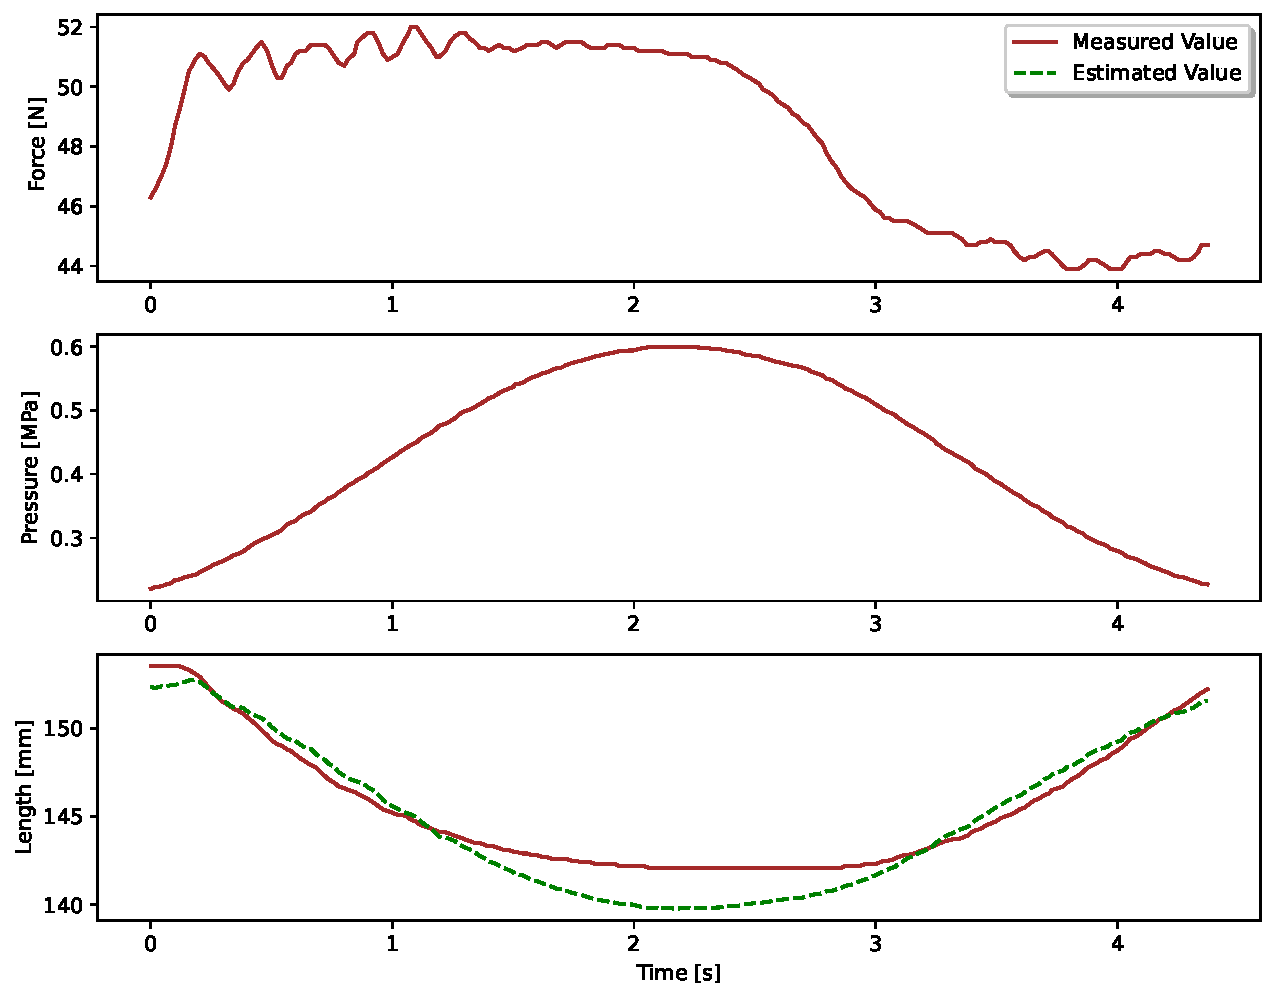
\includegraphics[width=\columnwidth]{fig/20231220_2_s_by_2_2d_ieeesensors1.pdf}
%    \caption{Dynamic length estimation (PAM-D, Silicon)}
%    \label{fig:pam_d_dynamic}
% \end{figure}

% \clearpage






% \begin{table}[h]
%     \centering
%     \caption{Maximum error and root mean squared \\percentage error of dynamic length estimation }
%     \resizebox{\columnwidth}{!}{
%         \begin{tabular}{c|cccccc}
%             \hline
%             PAM & \begin{tabular}[c]{@{}c@{}}Maximum Error[$\%$]\\(Eq.(\ref{eq:model})) \end{tabular} & \begin{tabular}[c]{@{}c@{}}Root Mean\\Squared Error[$\%$]\\(Eq.(\ref{eq:model})) \end{tabular} & \begin{tabular}[c]{@{}c@{}}Maximum Error[$\%$]\\(Eq.(\ref{eq:model_2d1})) \end{tabular} & \begin{tabular}[c]{@{}c@{}}Root Mean\\Squared Error[$\%$]\\(Eq.(\ref{eq:model_2d1})) \end{tabular}&\begin{tabular}[c]{@{}c@{}}Maximum Error[$\%$]\\(Eq.(\ref{eq:model_3d})) \end{tabular}& \begin{tabular}[c]{@{}c@{}}Root Mean\\Squared Error[$\%$]\\(Eq.(\ref{eq:model_3d}))\\
%             \hline \hline
%             A & 1.72&0.861&1.12&0.633& &&\\
%             B & 1.19&0.653 &0.773&0.353&&&\\
%             C & 1.18&0.683&1.01&0.548& &&\\
%             D & 1.65 & 0.846 &0.755& 0.435& &&\\
%             \hline
%             \hline
%         \end{tabular}
%     }
%     \label{tab:error}
% \end{table}

% \begin{table}[h]
%     \centering
%     \caption{Maximum error and root mean squared \\percentage error of dynamic length estimation }
%     \resizebox{\columnwidth}{!}{
%         \begin{tabular}{c|ccccccc}
%             \hline
%             PAM & \begin{tabular}[c]{@{}c@{}}Maximum Error[$\%$]\\(Eq.(\ref{eq:model})) \end{tabular} & \begin{tabular}[c]{@{}c@{}}Root Mean\\Squared Error[$\%$]\\(Eq.(\ref{eq:model})) \end{tabular} & \begin{tabular}[c]{@{}c@{}}Maximum Error[$\%$]\\(Eq.(\ref{eq:model_2d(1)})) \end{tabular} & \begin{tabular}[c]{@{}c@{}}Root Mean\\Squared Error[$\%$]\\(Eq.(\ref{eq:model_2d(1)})) \end{tabular}&\begin{tabular}[c]{@{}c@{}}Maximum Error[$\%$]\\(Eq.(\ref{eq:model_3d})) \end{tabular}&\begin{tabular}[c]{@{}c@{}}Root Mean\\Squared Error[$\%$]\\(Eq.(\ref{eq:model_3d})) \end{tabular} \\
%             \hline \hline
%             A & 1.72&0.861&1.12&0.633&1.22&0.516&\\
%             B & 1.19&0.653 &0.773&0.353&1.41&0.484&\\
%             C & 1.18&0.683&1.01&0.548&0.951&0.500&\\
%             D & 1.65 & 0.846 &0.755& 0.435&1.99&0.606&\\
%             \hline
%         \end{tabular}
%     }
%     \label{tab:error}
% \end{table}


% \subsection{推定パラメータ同定}
% 図\ref{fig:length_pressure}は,4種の空気圧人工筋の圧力$P$と自然長$L_n$の関係である.
% 仮定通り,圧力$P$に対して自然長$L_n$が線形的に減少する傾向が見られる.
% 図中の点線は,最小二乗法により各データ郡にフィッティングした(\ref{eq:L_n})式である.

% 一方,図\ref{fig:pam_b_static1}はPAM-Bに対する推定パラメータ同定実験の結果である.
% ただし,赤色の点が膨張時のデータ,青色の点が収縮時のデータ,緑色の点線が取得した推定パラメータ$a_i$による推定値を表す.
% 一般に,空気圧人工筋は摩擦によるヒステリシスを有するので,膨張時と収縮時でデータが異なる.
% % また,図\ref{fig:pam_b_static2}は図\ref{fig:pam_b_static1}中の5つの圧力に対する各データをまとめて三次元空間上に示した図である.
% 本論文では,紙幅上PAM-Bに対する実験結果のみ示すが,他の空気圧人工筋に対しても同様の結果が得られた.

% \begin{figure}[H]
%    \centering
%    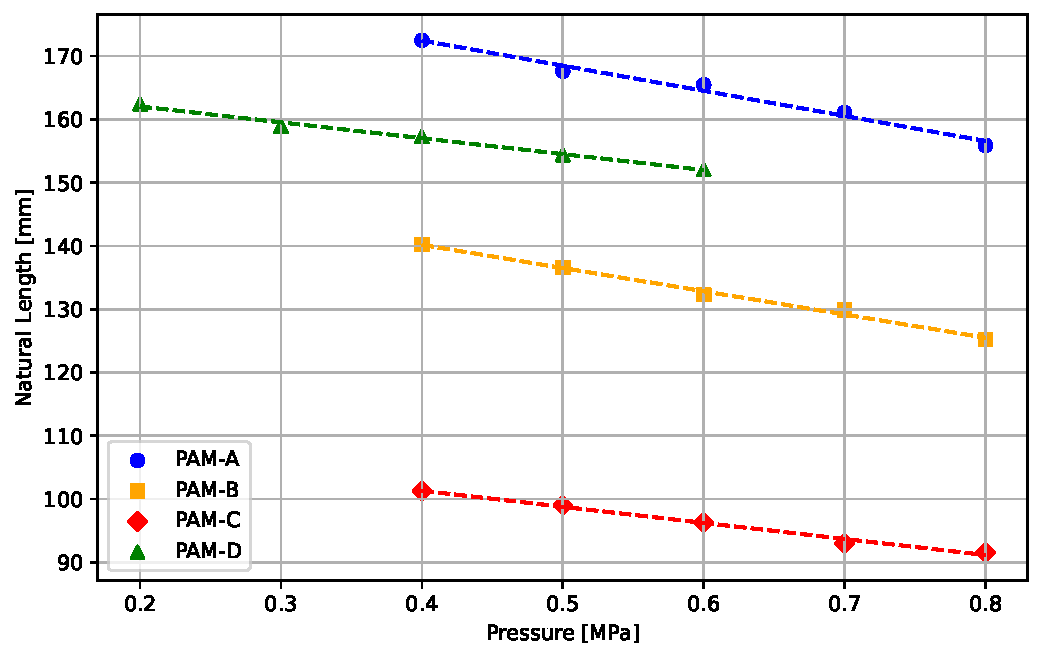
\includegraphics[width=\columnwidth]{fig/length_pressure.pdf}
%    \caption{Relationship between pressure and unstretched length}
%    \label{fig:length_pressure}
% \end{figure}

% \begin{figure}[H]
%    \centering
%    \includegraphics[width=\columnwidth]{fig/20231124_5_4s_se_2d_g.pdf}
%    \caption{Relationship between force and stretched length at each pressure (PAM-B)}
%    \label{fig:pam_b_static1}
% \end{figure}

% % \begin{figure}[H]
% %    \centering
% %    \includegraphics[width=\columnwidth]{fig/20231124_5_4s_se_3d_g.pdf}
% %    \caption{Relationship between pressure, force and stretched length (PAM-B)}
% %    \label{fig:pam_b_static2}
% % \end{figure}


% \subsection{動的測定実験} 
% 図\ref{fig:pam_b_dynamic}は,,PAM-Bに対して取得した推定パラメータを用い,動的に長さを推定した結果である.
% 提案手法では,表\ref{tab:error}の第2列および第3列に示す最大誤差および平均平方二乗誤差率で,それぞれ動的に長さを推定できた.


% \begin{figure}[H]
%    \centering
%    \includegraphics[width=\columnwidth]{fig/20231207_1_4s_by_5_2d_g.pdf}
%    \caption{Result of dynamic length estimation (PAM-B)}
%    \label{fig:pam_b_dynamic}
% \end{figure}

% \begin{table}[h]
%     \centering
%     \caption{Maximum error and root mean squared \\percentage error of dynamic length estimation }
%     \resizebox{\columnwidth}{!}{
%         \begin{tabular}{c|ccccc}
%             \hline
%             \begin{tabular}[c]{@{}c@{}}空気圧\\人工筋\end{tabular} & \begin{tabular}[c]{@{}c@{}}最大誤差[$\%$]\\(二次式) \end{tabular} & \begin{tabular}[c]{@{}c@{}}平均平方\\二乗誤差率[$\%$]\\(二次式) \end{tabular} & \begin{tabular}[c]{@{}c@{}}最大誤差[$\%$]\\(三次式) \end{tabular} & \begin{tabular}[c]{@{}c@{}}平均平方\\二乗誤差率[$\%$]\\(三次式) \end{tabular} \\
%             \hline \hline
%             PAM-A & 0.975&0.510&1.22&0.516& \\
%             PAM-B & 0.955&0.510 &1.41&0.484&\\
%             PAM-C & 1.07&0.580&0.951&0.500& \\
%             PAM-D & 1.41 & 0.475 &1.99& 0.606& \\
%             \hline
%         \end{tabular}
%     }
%     \label{tab:error}
% \end{table}
